\documentclass{article}
\usepackage[utf8]{inputenc}
\usepackage[margin=1in]{geometry}
\usepackage{amsmath}
\usepackage{graphicx}
\setlength{\parindent}{0em}
\setlength{\parskip}{0.5em}


\title{CTA200 2020 Assignment 2}
\author{Henri Lamarre}
\date{}

\begin{document}

\maketitle

\section{Question 1}
\subsection{Methods}
In this section, we initialize 100 randomly sampled points in the complex square of width 4 centered at $(0,0)$. We then iterate with the rule $z_{i+1}=z_i+c$. We then assign the color red to the points that end up outside the box at the end of the 20 iterations. We assign the color blue to the points that are still in the box after the 20 iterations. Then, we zoom on the square of width $0.2$ centered at $(0,0)$ and redo the same process.

\begin{figure}[h]
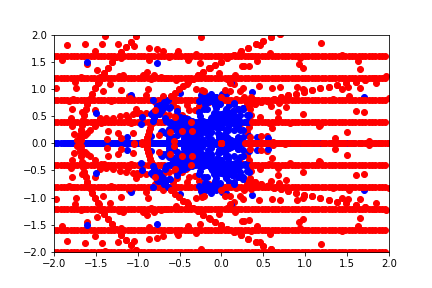
\includegraphics[width = 0.5\columnwidth]{question1_1.png}
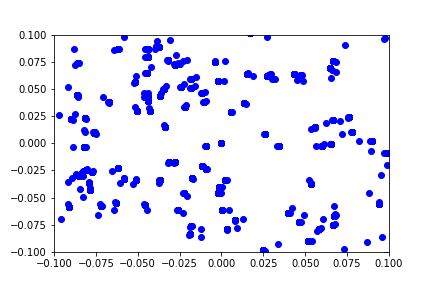
\includegraphics[width = 0.5\columnwidth]{question1_2.png}
\caption{[Left] Scatter plot of the positions of points for each iteration step in the box of width 4. [Right] Scatter plot of the positions of points for each iteration step in the box of width 0.2.}
\end{figure}


\subsection{Analysis}
We note that points that converge are mostly points which $|y|$ value is smaller than $0.5$. We then zoom on the square to make sure that that restriction is respected and indeed, all the points converge.


\section{Question 2}
\subsection{Methods}
We solve the set of first degree ODEs using scipy.integrate.odeint(). We supply the following initial conditions: 999 susceptibles, 1 infected and 0 recovered. Then, we modify one of the ODE and add a new one by introducing deaths in the parameter $\alpha$. We then use scipy again to solve these four ODEs.

\begin{figure}[h]
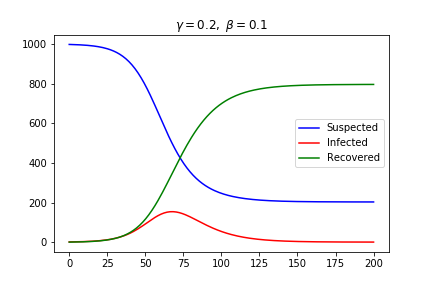
\includegraphics[width = 0.5\columnwidth]{question2_1.png}
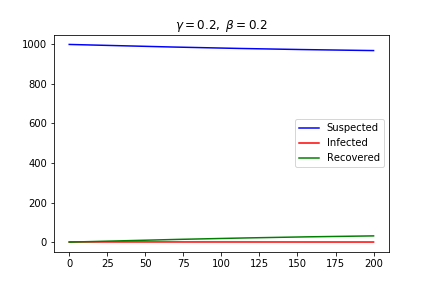
\includegraphics[width = 0.5\columnwidth]{question2_2.png}
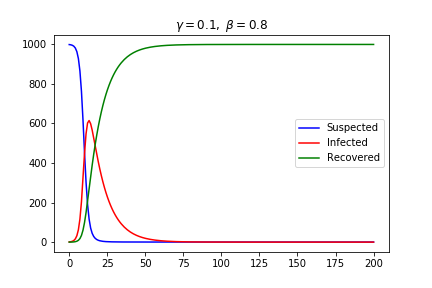
\includegraphics[width = 0.5\columnwidth]{question2_3.png}
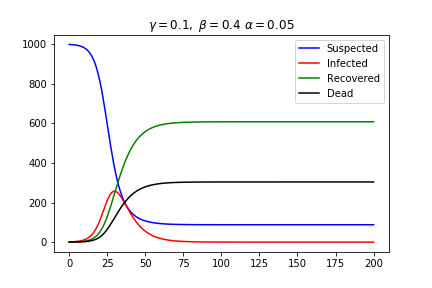
\includegraphics[width = 0.5\columnwidth]{question2_4.png}
\caption{Evolution of the number of people in the groups: Infected, Susceptible (Suspected), Recovered and Dead. The parameter $\alpha$ is 0 in the first three plots.}
\end{figure}

\subsection{Analysis}
By increasing $\beta$, the rate of propagation is substancially lowered. We hypothesise that $\beta$ is inversly proportionnal to the rate of propagation of the virus. Then, by increasing $\gamma$, we notice that more people get infected. We hypothesise that $\gamma$ is related to the chances of contracting the virus by being in contact with it. Then, by adding the death parameter, we notice that the number of infected decreases faster which was expected.


\end{document}
